\documentclass[11pt,a4paper,UTF8]{ctexart}

%%%%%%===== 宏包调用 =====
\usepackage{CJK,CJKnumb,CJKspace}
\usepackage{graphicx}           % 插入图片
\usepackage{color}              % 支持彩色
\usepackage{indentfirst}        % 首行缩进宏包
\usepackage{amsmath,amssymb,bm} % AMS math宏包与数学符号加粗
\usepackage{cases}              % 数学公式
\usepackage{amssymb}
\usepackage{adjustbox}			%调整表格大小
\usepackage{cmap}				%解决pdf粘贴乱码
\usepackage{booktabs}			%绘制三线表
\usepackage[CJKbookmarks=true, colorlinks=true]{hyperref}			%插入链接

%%%%%%===== 重定义字体和字号 =====
\newcommand{\song}{\CJKfamily{song}}    % 宋体
\newcommand{\fs}{\CJKfamily{fs}}        % 仿宋体
\newcommand{\kai}{\CJKfamily{kai}}      % 楷体
\newcommand{\hei}{\CJKfamily{hei}}      % 黑体
\newcommand{\li}{\CJKfamily{li}}        % 隶书
\newcommand{\chuhao}{\fontsize{42pt}{\baselineskip}\selectfont}     % 初号
\newcommand{\xiaochuhao}{\fontsize{36pt}{\baselineskip}\selectfont} % 小初号
\newcommand{\yihao}{\fontsize{28pt}{\baselineskip}\selectfont}      % 一号
\newcommand{\xiaoyihao}{\fontsize{24pt}{\baselineskip}\selectfont}  % 小一号
\newcommand{\erhao}{\fontsize{21pt}{\baselineskip}\selectfont}      % 二号
\newcommand{\xiaoerhao}{\fontsize{18pt}{\baselineskip}\selectfont}  % 小二号
\newcommand{\sanhao}{\fontsize{16pt}{\baselineskip}\selectfont}     % 三号
\newcommand{\xiaosanhao}{\fontsize{15pt}{\baselineskip}\selectfont} % 小三号
\newcommand{\sihao}{\fontsize{14pt}{\baselineskip}\selectfont}      % 四号
\newcommand{\xiaosihao}{\fontsize{12pt}{\baselineskip}\selectfont}  % 小四号
\newcommand{\wuhao}{\fontsize{10.5pt}{\baselineskip}\selectfont}    % 五号
\newcommand{\xiaowuhao}{\fontsize{9pt}{\baselineskip}\selectfont}   % 小五号

%%%%%%===== 页面设置 =====
\setlength{\textwidth}{14.5cm}  % 正文宽度
\setlength{\textheight}{20cm}   % 正文高度
\setlength{\hoffset}{0cm}       % 左边距 = \hoffset + 1 英寸
\setlength{\voffset}{0cm}       % 顶端距离 = \voffset + 1 英寸
\setlength{\parskip}{3pt plus1pt minus1pt}  % 段落之间的竖直距离
\renewcommand{\baselinestretch}{1.2}    % 定义行距
\setlength{\parindent}{0pt} %首行顶格
%%%%%%===== 自定义命令 =====
\numberwithin{equation}{section}

\begin{document}
\song
\CJKindent\CJKtilde

%%%%%%===== 图片文件夹指定 =====
\graphicspath{{figures/}}

%%%%%%===== 标题名称中文化 =====
\renewcommand\abstractname{\hei 摘\ 要}
\renewcommand\refname{\hei 参考文献}
\renewcommand\figurename{\hei 图}
\renewcommand\tablename{\hei 表}
\newtheorem{definition}{\hei 定义~}[section]
\newtheorem{theorem}{\hei 定理~}[section]
\newtheorem{lemma}[theorem]{\hei 引理~}
\newtheorem{corollary}[theorem]{\hei 推论~}
\newtheorem{proposition}[theorem]{\hei 命题~}

\title{一种解决车辆路径和卡车司机调度的精确解法\thanks{原论文\cite{test}}}
\author{light\\学号~xxxxxx, 专业}
\date{2017~年~2~月~7~日}
\maketitle 

%生成目录,可以选择不生成
\tableofcontents

\begin{abstract}
本论文研究的是关于车辆路径和卡车司机调度(VRTDSP)的问题。建立了适用于不同运输规则下的模型,并且使用分支定价算法进行求解和证明问题的解是否为最优解。其意义不仅在于这是第一个解决VRTDSP并且证明最优性的算法而且运用研究成果漂亮地解决了实际问题。
\end{abstract}


\section{应用背景描述}
\label{sec:background}
对于长距离的运输,如果卡车司机长时间驾驶而不定期进行休息,就会产生很大发生事故的风险。因此,政府制订了一系列的政策来保证驾驶的安全。以美国政府为例,驾驶员在没有连续休息10小时情况下不能连续驾驶11小时;驾驶员在休息后不能连续驾驶14小时;驾驶员在至少休息30分钟情况下不能连续驾驶8小时;break不能少于30分钟。
	
在这一系列限制下面,运输公司期望规划最优的路径,以减小运输的成本。由于美国制定的新运输规定,以前的一些解法不在这些约束条件下规划路径,所以不适用新运输规定下的路径规划。而且目前并没有一种在以上问题背景下的精确解法。文章提出了一种高效的标签算法,并且建模证明了其可行性,使用分支定价的方法进行求解。

\subsection{数学建模描述}
\label{sec:math_model}
VRTDSP可以转化为带时间窗的车辆路径规划问题(VRPTW)。模型变量如下
\begin{itemize}
	\item $C$~:~顾客集合
	\item $n^{depot}$~:~仓库的集合
	\item $N=C\cup n^{depot}$~:~卡车可以经过的节点
	\item $\left[t_{n}^{min}, t_{n}^{max}\right]$~:~经过节点$n$的时间窗,其中$n\in C$
	\item $q_n$~:~节点$n$的货物需求
	\item $s_n$~:~节点$n$的服务时间
	\item $c_{nm}$~:~运输成本,其中$\left(n,m\right) \in A $
	\item $d_{nm}$~:~运输时间,其中$\left(n,m\right) \in A $
	\item $Q$~:~卡车的运输货物容量,假设每辆卡车容量相同
	\item $r=\left(n_0,n_1,\ldots,n_{k-1},n_k\right)$~:~运输的路线
	\item $G=\left(N,A\right)$~:~运输的网络
\end{itemize}

规划的问题\ref{eq:target}:
\begin{subequations}
\begin{align}
	\min &\sum_{r\in R}{c_r \times x_r} \\
	\text{s.t.} &\sum_{r\in R}{a_{nr}x_r}=1 \text{ for all }n \in C \\
	& x_r \in \left\{ 0, 1\right\}
\end{align}
\label{eq:target}
\end{subequations}

其中$R$是可行路径集合,$r\in R$。受到表x运输政策的约束...


流程如图\ref{fig:Branch_and_price_diagram}

\begin{figure}[hbt]
	\centering
	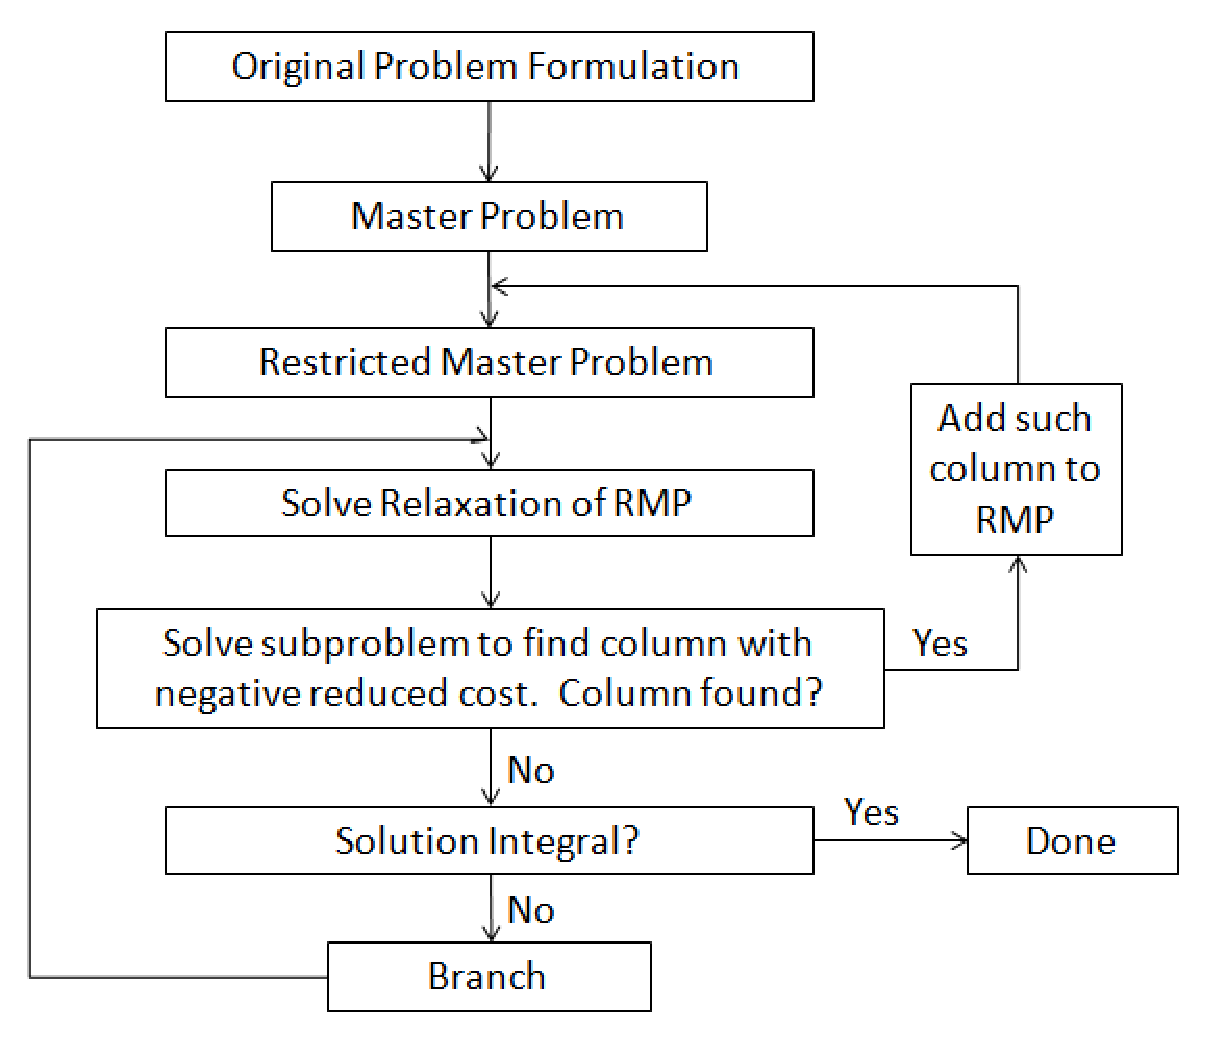
\includegraphics[width=0.6\textwidth]{branch_and_price_diagram}
	\caption{分支定价法流程图}
	\label{fig:Branch_and_price_diagram}
\end{figure}


% 参考文献
\clearpage
\bibliographystyle{IEEEtran}
\bibliography{citation}

\clearpage
\end{document}
